\chapter{Evaluation}
Evaluating an artistic project is difficult as there is a need to separate
aesthetic goals from more technical ones. Testing against the objectives I set
in the introduction may be potentially \emph{subjective} due to the nature of
the project. For example, how can we test if the program ``Allows the user to
experience the works of Viner'', for this some comparison of the methods used in
this project, the possibilities of the images they generate, and the existing
work of Viner needs to be made. User testing is possible to compare against the
user interaction elements, but would not tell the whole story of the more
artistic style.

I have therefore tried to talk about some of the more aesthetic goals and
evaluate them as technically as possible, but with respect to the original
objectives.

\section{Reproduction of Viner's Style}
%TODO prove this?
The program cannot reproduce every image that Viner's pen plotter pieces span.
Ultimately this is due to fundamental design decisions in how the program
operates. For example, some of Viner's work includes non-closed polygons the
method outlined in \autoref{Polygons} cannot produce polygons that are not
closed. 

\begin{figure}[H]
    \centering
    \includegraphics[width=0.7\textwidth]{vinerimpossible}
    \caption{An example of an image that the program cannot reproduce}
\end{figure}

Some of Viner's work contains artefacts from the pen plotter method, which is
also not represented in the final program. This is an example of the medium and
the process he worked with, even if it was not ideal. Perhaps a program that
truly sought to reproduce the totality of his work should reproduce this as
well. Later plotter art by Viner also took on a radically different style, which
isn't explored in this project either.

\begin{figure}[H]
    \centering
    \begin{subfigure}[t]{0.49\textwidth}
        \centering
        \includegraphics[width=1\textwidth]{vinerbunching}
        \caption{`Bunching' at the bottom of the page, likely due to coordinates
        greater than that of the plotter's maximum range}
    \end{subfigure}
    \hfill
    \begin{subfigure}[t]{0.49\textwidth}
        \centering
        \includegraphics[width=1\textwidth]{laterplotter}
        \caption{An example of Viner's later pen plotter work}
    \end{subfigure}
    \caption{}
\end{figure}

This is not necessarily a failure outright, but does bare mentioning that the
program only explores a subset of Viner's work; which still provides the user
with the sense of exploring a possible `landscape' of which these images are
part of.

Fixing this would require some fundamental reworking to the way the graphics are
generated, perhaps creating the grid as a set of points and finding a way to
work out if the points should be drawn or lines between points should be drawn.

\section{Methods Used}
I believe that the methods outlined in \autoref{landgen} and
\autoref{Music} (specifically: \autoref{sonicnav} and
\autoref{Sequencing}) were successful in the sense that they are tools that
could be reused in any project.

The methods for auditory location outlined in \autoref{sonicnav} are of interest
to me to develop further as I believe they could be expanded to work well with
existing data visualisation programs and perhaps be used as a novel way to
explore multi-variate datasets as an extra part of, for example the grand tour
method as in \citep{asimov1985grand}; a chord could play with the intervals
marking the subsets you are viewing and move between chords as the image on the
screen changes. More exploration could also be completed with rhythm which is a
good use of temporal data, perhaps using `beats' as marks on a `ruler' in space
you are travelling through in time, with acceleration these beats get closer
together.

The noise `approximate rounding' method in \autoref{landgen} is an example of a
technique that can be fully integrated into another project at will, this was
successful example of creating a technique that is applicable to other projects.

\section{Navigation}
% is a sense of landscape there, does the user understand the concept?
<insert user results here>

\section{Audio}
% personal feelings, does it fit, does the user think it relates to the concept
% intuitively?
<insert user results here>

From an artistic perspective I think that the musical aspect was a success, this
is hard to evaluate as it is totally disconnected from even Viner's work.
Ideally I would have included some more depth. I had looked into using various
field recordings from around Leeds I have made as backing for the music but the
technical aspects of this made it impossible to implement without using a
web server meaning the whole application was less portable.

\begin{figure}[H]
    \centering
    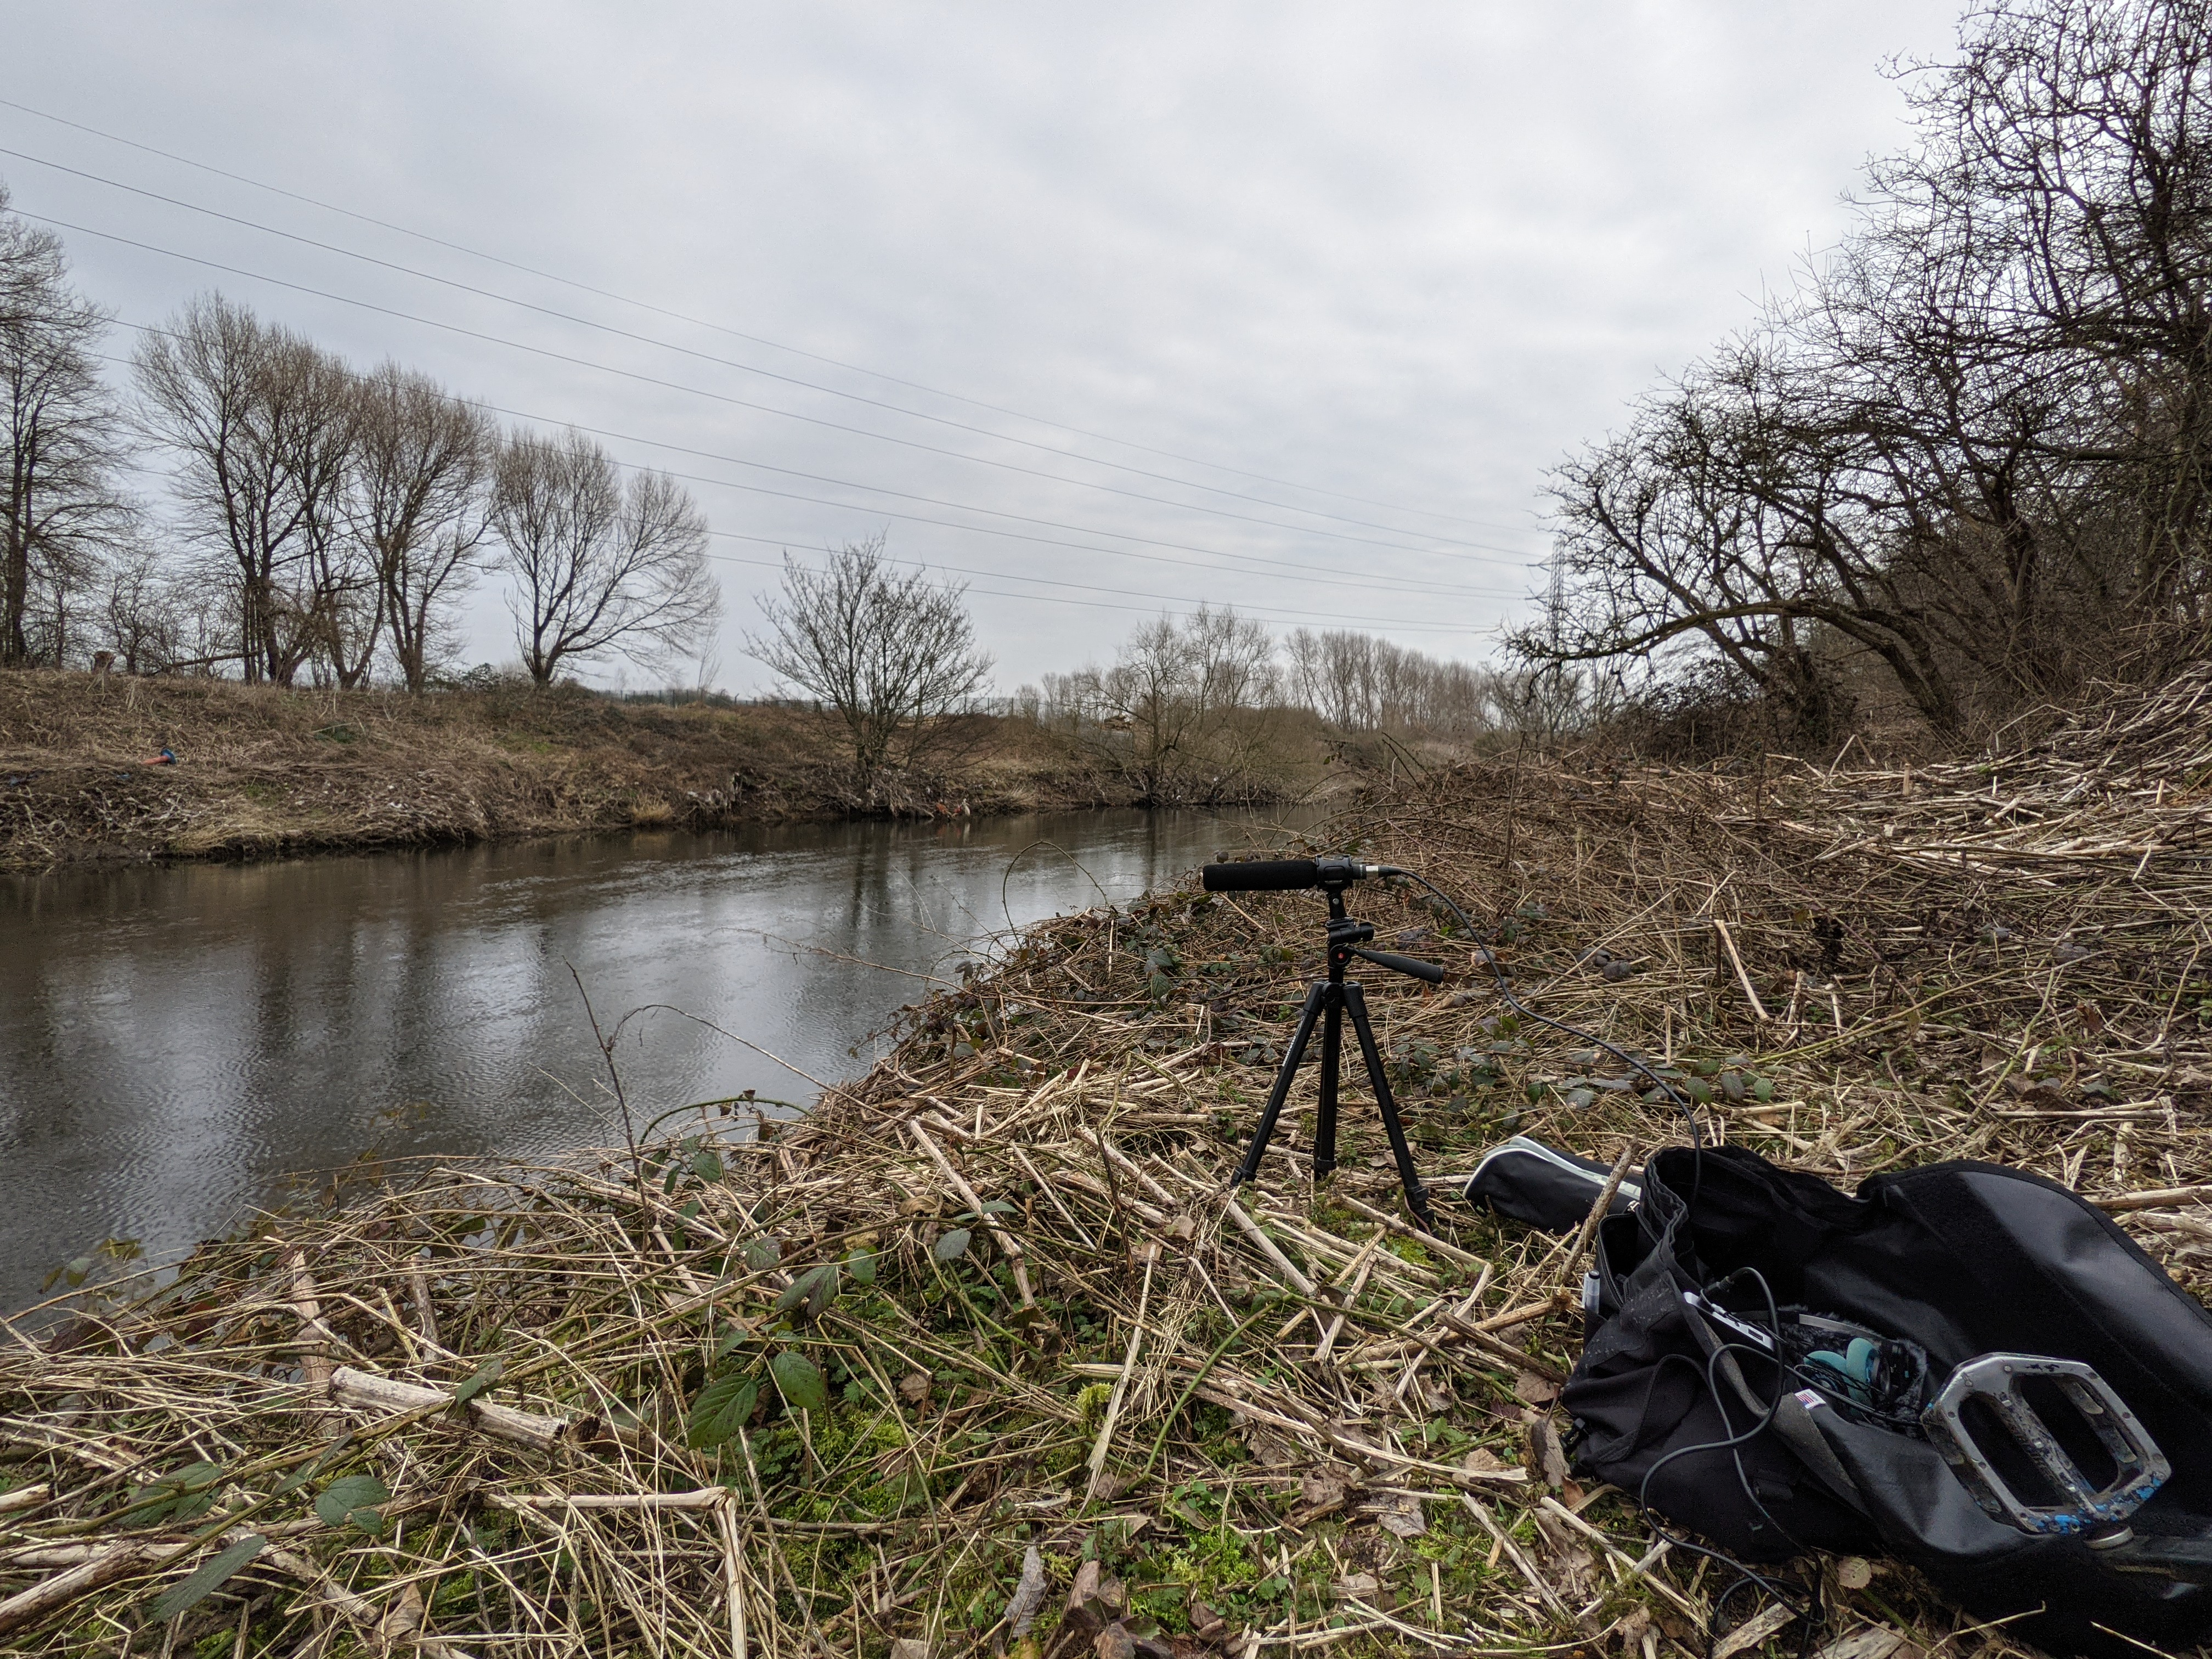
\includegraphics[width=0.5\textwidth]{fieldrecording}
    \caption{Field recording setup}
\end{figure}

\section{History}
% is the history intuitive, does it work how the user expects it to work?
<insert user results here>
